\documentclass[slidetop,11pt]{beamer}
%
% Ces deux lignes {\`a} d{\'e}commenter pour sortir 
% le texte en classe article
% \documentclass[class=article,11pt,a4paper]{beamer}
% \usepackage{beamerbasearticle}

% Packages pour les fran\c{c}ais
%
\usepackage[T1]{fontenc} 
\usepackage[latin1]{inputenc}
\usepackage[frenchb]{babel}
% pour un pdf lisible {\`a} l'{\'e}cran si on ne dispose pas 
% des fontes cmsuper ou lmodern
%\usepackage{lmodern}
\usepackage{aeguill}

% Pour afficher le pdf en plein ecran
% (comment{\'e} pour imprimer les transparents et pour les tests)
%\hypersetup{pdfpagemode=FullScreen}

% ------------------------------------------------
%-----------   styles pour beamer   --------------
% ------------------------------------------------
%
% ------------- Choix des couleurs ---------------

%% %% %% %% %% COULEURS PERSOS
\definecolor{verylightblack}{rgb}{0.25,0.25,0.25}
\definecolor{lightblack}{rgb}{0.1,0.1,0.1}
\definecolor{black}{rgb}{0,0,0}


\definecolor{verylightgrey}{rgb}{0.8,0.8,0.8}
\definecolor{lightgrey}{rgb}{0.6,0.6,0.6}
\definecolor{grey}{rgb}{0.4,0.4,0.4}

\definecolor{verylightgray}{gray}{0.80}
\definecolor{lightgray}{gray}{0.6}
\definecolor{gray}{gray}{0.4}

\definecolor{verylightblue}{rgb}{0.9,0.9,1.0}
\definecolor{lightblue}{rgb}{0.75,0.75,1.0}
\definecolor{blue}{rgb}{0.5,0.5,1.0}
\definecolor{darkblue}{rgb}{0.0,0.0,0.5}

\definecolor{verylightred}{rgb}{1.0,0.9,0.9}
\definecolor{lightred}{rgb}{1.0,0.75,0.75}
\definecolor{red}{rgb}{1.0,0.5,0.5}

\definecolor{verylightgreen}{rgb}{0.9,1.0,0.9}
\definecolor{lightgreen}{rgb}{0.75,1.0,0.75}
\definecolor{green}{rgb}{0.5,1.0,0.5}


\definecolor{verylightcolorUN}{rgb}{1.0,0.75,1.0}
\definecolor{lightcolorUN}{rgb}{1.0,0.50,1.0}

\definecolor{verylightcolorDE}{rgb}{0.75,1.0,1.0}
\definecolor{lightcolorDE}{rgb}{0.50,1.0,1.0}

\definecolor{verylightcolorTR}{rgb}{1.0,1.0,0.75}
\definecolor{lightcolorTR}{rgb}{1.0,1.0,0.50}


% Red{\'e}finit la couleur de fond pour imprimer sur transparents
%\xdefinecolor{fondtexte}{rgb}{1,1,1}     % blanc

% commande differente pour les couleurs nomm{\'e}es - de base
%\colorlet{coultexte}{black} 

% -------------- Fioritures de style -------------
% Fait afficher l'ensemble du frame 
% en peu lisible (gris clair) d{\`e}s l'ouverture
\beamertemplatetransparentcovered

% Supprimer les icones de navigation (pour les transparents)
%\setbeamertemplate{navigation symbols}{}

% Mettre les icones de navigation en mode vertical (pour projection)
%\setbeamertemplate{navigation symbols}[vertical]

% ------------ Choix des th{\`e}mes ------------------
\usecolortheme{default} % gabywald
% \usecolortheme{orchid}

\setbeamercolor{title}{fg=black, bg=blue!40}
\setbeamercolor{block title}{fg=black, bg=blue!40}
\setbeamercolor{structure}{fg=black, bg=blue!40}
\setbeamercolor{block title}{fg=black, bg=lightblue!40}
\setbeamercolor{substructure}{fg=black, bg=verylightblue!40}

\setbeamercolor{block title UN}{fg=black, bg=lightcolorUN!40}
\setbeamercolor{substructureUN}{fg=black, bg=verylightcolorUN!40}

\setbeamercolor{block title DE}{fg=black, bg=lightcolorDE!40}
\setbeamercolor{substructureDE}{fg=black, bg=verylightcolorDE!40}

\setbeamercolor{block title TR}{fg=black, bg=lightcolorTR!40}
\setbeamercolor{substructureTR}{fg=black, bg=verylightcolorTR!40}

% \setbeamercolor{block title}{fg=black, bg=lightblue!40}
% \setbeamercolor{block body}{...}
% \setbeamercolor{block title example}{...}
% \setbeamercolor{block body example}{...}
% \setbeamercolor{block title alerted}{...}
% \setbeamercolor{block body alerted}{...}

% \useoutertheme[left]{sidebar}
% \setbeamersize{sidebar left width=3.0cm \tableofcontents[hideothersubsections] }
% \setbeamercolor{sidebar left}{fg=green,bg=lightgreen}
% \setbeamercolor{title in sidebar}{parent=title}

\setbeamercolor*{sidebar}{fg=lightblack,bg=lightblue!75!white}

\setbeamercolor*{palette sidebar primary}{fg=darkblue!50!lightgrey}
\setbeamercolor*{palette sidebar secondary}{fg=black} % darkblue!10!black
\setbeamercolor*{palette sidebar tertiary}{fg=darkblue!50!lightgrey}
\setbeamercolor*{palette sidebar quaternary}{fg=black} % darkblue!10!black

\setbeamercolor{subsubsection in sidebar}{hideallsubsections}
\setbeamercolor{subsubsection in sidebar shaded}{hideallsubsections}


%------------ fin style beamer -------------------

% Faire appara{\^i}tre un sommaire avant chaque section
% \AtBeginSection[]{
%   \begin{frame}
%   \frametitle{Plan}
%   \medskip
%   %%% affiche en d{\'e}but de chaque section, les noms de sections et
%   %%% noms de sous-sections de la section en cours.
%   \small \tableofcontents[currentsection, hideothersubsections]
%   \end{frame} 
% }

% ----------- Contenu de la page de titre --------
\title{Gestion de Projet, Traitements de donn{\'e}es...}
\subtitle{Conception, D{\'e}veloppement, Tests et Production}
% \author{Gabriel Chandesris}
% \institute{Universit{\'e} de Barrayar}
\institute{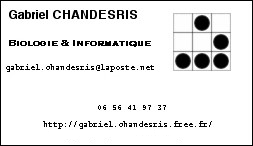
\includegraphics[width=5cm]{img/cartevisite.png}}
\date{08 Novembre 2010}
%% \logo{
\includegraphics[height=0.5cm]{img/logo_glider.png}}

% ----------- Nom des diff{\'e}rentes parties --------
\def\sectionPartII{Pr{\'e}sentation Perso}
\def\sectionPartIIa{Parcours de formation}
\def\sectionPartIIaUN{BTS Biochimie (2003)}
\def\sectionPartIIaDE{Licence Bio-Informatique au CNAM (2005 -- 2007)}
\def\sectionPartIIaTR{IUP GBI {\`a} Evry - Genopole (2009)} %% \copyright
\def\sectionPartIIb{Parcours professionnel}
\def\sectionPartIIbUN{Laboratoires, H{\^o}pitaux...}
\def\sectionPartIIbDE{Recherche Publique}
\def\sectionPartIIbTR{Recherche Priv{\'e}e / Industrie}
\def\sectionPartIIc{Projets}
\def\sectionPartIIcUN{Mod{\'e}lisation Biologique}
\def\sectionPartIIcDE{Simulation Informatique}
\def\sectionPartIIcTR{Un soup\c{c}on de 3D...}


\def\sectionPartI{Axes principaux}
\def\sectionPartIa{Gestion de projet}
\def\sectionPartIaUN{Conception (R{\'e}flexion et UML...) -- }
\def\sectionPartIaDE{D{\'e}veloppement et tests}
\def\sectionPartIaTR{D{\'e}ploiement ([Pr{\'e}-]Production)}
\def\sectionPartId{Outils et M{\'e}thodes}
\def\sectionPartIdUN{Outils (IDE : Eclipse et {\'e}quivalents, Qualit{\'e})}
\def\sectionPartIdDE{M{\'e}thodes (eXtreme Prog. , Agilit{\'e}, Plannings)}
\def\sectionPartIdTR{Int{\'e}r{\^e}ts : Prototypage ET Industrialisation !}
\def\sectionPartIb{Traitements De Donn{\'e}es}
\def\sectionPartIbUN{Formats De Donn{\'e}es}
\def\sectionPartIbDE{Bases De Donn{\'e}es}
\def\sectionPartIbTR{Autres...}
\def\sectionPartIc{Programmation}
\def\sectionPartIcUN{Imp{\'e}ratif / Fonctionnel}
\def\sectionPartIcDE{Orient{\'e} Objet (POO)}
\def\sectionPartIcTR{Autres...}


\def\sectionPartIII{<<Pack Bonus>>}
\def\sectionPartIIIa{Information !!}
\def\sectionPartIIIaUN{InterWeb et Librairies}
\def\sectionPartIIIaDE{E-Mail et NewsGroup / Forum}
\def\sectionPartIIIaTR{Veille Info / Techno}
\def\sectionPartIIIb{Hackez !! (bidouille)}
\def\sectionPartIIIbUN{Ma{\^i}tre devenu tu es, Padawan tu restes...}
\def\sectionPartIIIbDE{Participation {\`a} des projets}
\def\sectionPartIIIbTR{Biologie ++ Informatique}
\def\sectionPartIIIc{Prospective}
\def\sectionPartIIIcUN{R{\'e}formes (l{\'e}gislatives, sociales)...}
\def\sectionPartIIIcDE{Investissements Industriels}
\def\sectionPartIIIcTR{Initiative(s)...}

\def\sectionPartIV{Questions}
\def\sectionPartIVa{Le Libre et l'OpenSource}
\def\sectionPartIVb{Outils pratiques Unix / Linux / ...}
\def\sectionPartIVc{Recherche d'emploi et code du travail}
\def\sectionPartIVd{"Social Patterns"}
\def\sectionPartIVe{...}

\def\moreInFrameTitle{
\includegraphics[height=0.5cm]{img/logo_glider.png}~~~~~}

% ------------------------------------------------
% -------------   D{\'e}but document   ---------------
% ------------------------------------------------
\begin{document}
%--------- {\'e}criture de la page de titre ----------
% avec la commande frame simplifi{\'e}e
\frame[plain]{\titlepage}
%

%------------------ Sommaire ---------------

\begin{frame}
	\frametitle{\moreInFrameTitle Sommaire}
	\small \tableofcontents[hideallsubsections]
\end{frame} 


%***************************************
%******     II Pr{\'e}sentation  *******
%***************************************
\section{\sectionPartII}
\begin{frame}
	\frametitle{\moreInFrameTitle \sectionPartII}
	\tableofcontents[sections=1,subsectionstyle=shaded/shaded/shaded]
\end{frame} 

\subsection{\sectionPartIIa}
\begin{frame}
	\frametitle{\moreInFrameTitle \sectionPartIIa}
	\tableofcontents[sections=1,subsectionstyle=show/shaded/hide]
\end{frame}

\subsubsection{\sectionPartIIaUN}
\begin{frame}
	\frametitle{\moreInFrameTitle \sectionPartIIaUN}
	\begin{columns}[T]
	\begin{column}[T]{5cm}
		
\includegraphics[height=5cm]{img/fondcote.png}
	\end{column}
	\begin{column}[T]{7cm}
		 \begin{beamerboxesrounded}	[lower=substructureUN, %
		 				 upper=block title UN,%
						 shadow=true]%
		       {\sectionPartIIaUN}
			\begin{itemize}
				\item Biochimie / chimie organique... 
				\item Bact{\'e}riologie / Microbiologie... 
				\item Immunologie, contr{\^o}les qualit{\'e}... 
				\item Techniques classiques et Automates d'analyses...
				\item Autant de th{\'e}orie que de pratique !!
			\end{itemize}
		\end{beamerboxesrounded}
	\end{column}
	\end{columns}
\end{frame}

\subsubsection{\sectionPartIIaDE}
\begin{frame}
	\frametitle{\moreInFrameTitle \sectionPartIIaDE}
	\begin{columns}[T]
	\begin{column}[T]{7cm}
		\begin{beamerboxesrounded}	[lower=substructureDE, %
		 				 upper=block title DE,%
						 shadow=true]%
		       {\sectionPartIIaDE}
			\begin{itemize}
				\item \textbf{Cours du soir}, Conservatoire National des Arts et M{\'e}tiers. 
				\item Remise {\`a} plat des concepts d'algorithmique et de programmation (Scheme -- LISP, JAVA). 
				\item Contacts professionnels (pas seulement universitaires). 
				\item Ax{\'e} outils de bio-informatique. 
			\end{itemize}
		\end{beamerboxesrounded}
	\end{column}
	\begin{column}[T]{3cm}
		
\includegraphics[height=5cm]{img/logo_cnam.png}
	\end{column}
	\end{columns}
\end{frame}

\subsubsection{\sectionPartIIaTR}
\begin{frame}
	\frametitle{\moreInFrameTitle \sectionPartIIaTR}
	\begin{columns}[T]
	\begin{column}[T]{5cm}
		
\includegraphics[height=4cm]{img/logo_ueve_2010.png}
	\end{column}
	\begin{column}[T]{7cm}
		\begin{beamerboxesrounded}	[lower=substructureTR, %
		 				 upper=block title TR,%
						 shadow=true]%
		       {\sectionPartIIaTR}
			\begin{itemize}
				\item \emph{...}
				\item Tr{\`e}s (trop) universitaire. 
				\item Ne pas h{\'e}siter {\`a} voir {\`a} c{\^o}t{\'e} (pure info. et pure biologie). 
				\item Les stages sont des plus (++) non n{\'e}gligeables {\`a} consid{\'e}rer comme exp{\'e}rience pro. !!
			\end{itemize}
		\end{beamerboxesrounded}
	\end{column}
	\end{columns}
\end{frame}

\subsection{\sectionPartIIb}
\begin{frame}
	\frametitle{\moreInFrameTitle \sectionPartIIb}
	\tableofcontents[sections=1,subsectionstyle=show/shaded/hide]
\end{frame}

\subsubsection{\sectionPartIIbUN}
\begin{frame}
	\frametitle{\moreInFrameTitle \sectionPartIIbUN}
	\begin{columns}[T]
	\begin{column}[T]{5cm}
		
\includegraphics[width=4cm]{img/logo_aphp.png}~\\
		
\includegraphics[width=3cm]{img/logo_hia_begin.png}~\\
	\end{column}
	\begin{column}[T]{7cm}
		\begin{beamerboxesrounded}	[lower=substructureTR, %
		 				 upper=block title TR,%
						 shadow=true]%
		       {\sectionPartIIbUN}
			\begin{itemize}
				\item Militaire, priv{\'e}, public. 
				\item Sant{\'e} "g{\'e}n{\'e}rale" (public / semi-public > priv{\'e} : "raret{\'e}"). 
				\item Gestion particuli{\`e}re, convention et contr{\^o}le...
				\item Techniques automatis{\'e}es. 
			\end{itemize}
		\end{beamerboxesrounded}
	\end{column}
	\end{columns}
\end{frame}

\subsubsection{\sectionPartIIbDE}
\begin{frame}
	\frametitle{\moreInFrameTitle \sectionPartIIbDE}
	\begin{columns}[T]
	\begin{column}[T]{7cm}
		\begin{beamerboxesrounded}	[lower=substructureUN, %
		 				 upper=block title UN,%
						 shadow=true]%
		       {\sectionPartIIbDE}
			\begin{itemize}
				\item CNRS : IBISC, Evry
				\item Professeurs de l'IUP GBI et du CNAM. 
				\item ...
			\end{itemize}
		\end{beamerboxesrounded}
	\end{column}
	\begin{column}[T]{3cm}
		
\includegraphics[height=3cm]{img/logo_cnrs.png}
	\end{column}
	\end{columns}
\end{frame}

\subsubsection{\sectionPartIIbTR}
\begin{frame}
	\frametitle{\moreInFrameTitle \sectionPartIIbTR}
	\begin{columns}[c]
	\begin{column}[c]{5cm}
		
\includegraphics[width=4cm]{img/logo_sanofiaventis_FR.png}~\\~\\
		
\includegraphics[width=3cm]{img/logo_dassault_systemes_16_09_2009_13_50_26.png}~\\~\\
		
\includegraphics[width=2cm]{img/logo_edd.png}
	\end{column}
	\begin{column}[c]{7cm}
		 \begin{beamerboxesrounded}	[lower=substructureDE, %
		 				 upper=block title DE,%
						 shadow=true]%
		       {\sectionPartIIbTR}
			\begin{itemize}
				\item Sanofi-Aventis (Pharmacie): {\'e}tudes cliniques, g{\'e}n{\'e}tiques, brevets...
				\item Dassault Syst{\`e}mes (PLM, a{\'e}ronautique, automobile...) : 
				\begin{itemize} 
					\item Extension vers les Sciences de la Vie. 
					\item Projet BioIntelligence (socle + partenaires). 
				\end{itemize}
				\item EDD (traitement de donn{\'e}es des entreprises et de la presse). 
			\end{itemize}
		\end{beamerboxesrounded}
	\end{column}
	\end{columns}
\end{frame}

\subsection{\sectionPartIIc}
\begin{frame}
	\frametitle{\moreInFrameTitle \sectionPartIIc}
	\tableofcontents[sections=1,subsectionstyle=show/shaded/hide]
\end{frame}

\subsubsection{\sectionPartIIcUN}
\begin{frame}
	\frametitle{\moreInFrameTitle \sectionPartIIcUN}
	\begin{center}
	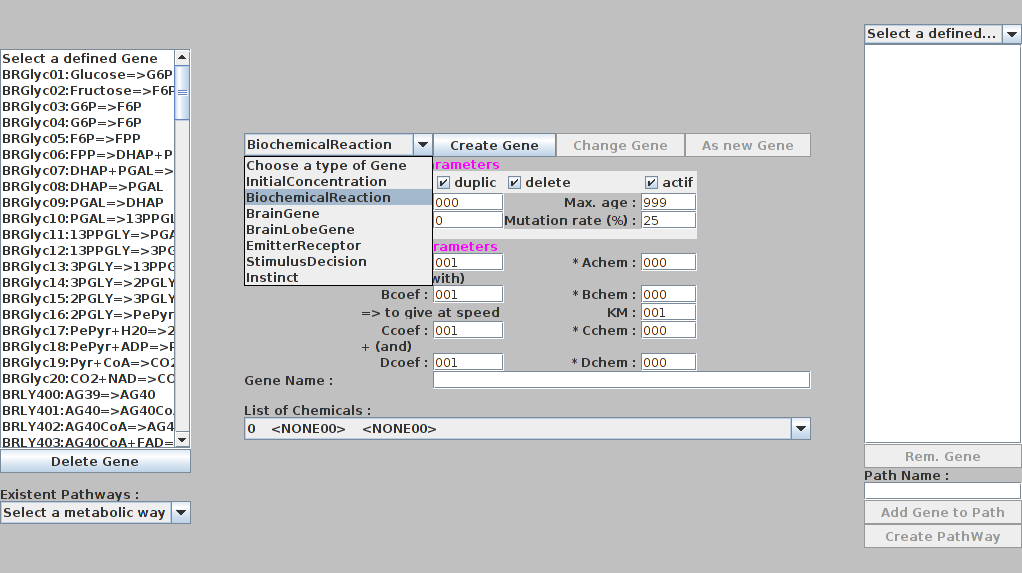
\includegraphics[height=6.5cm,width=11.6cm]{img/persoGeneCreatorGUI.png} 
	\end{center}
	% \vfill
	% \null\hfill 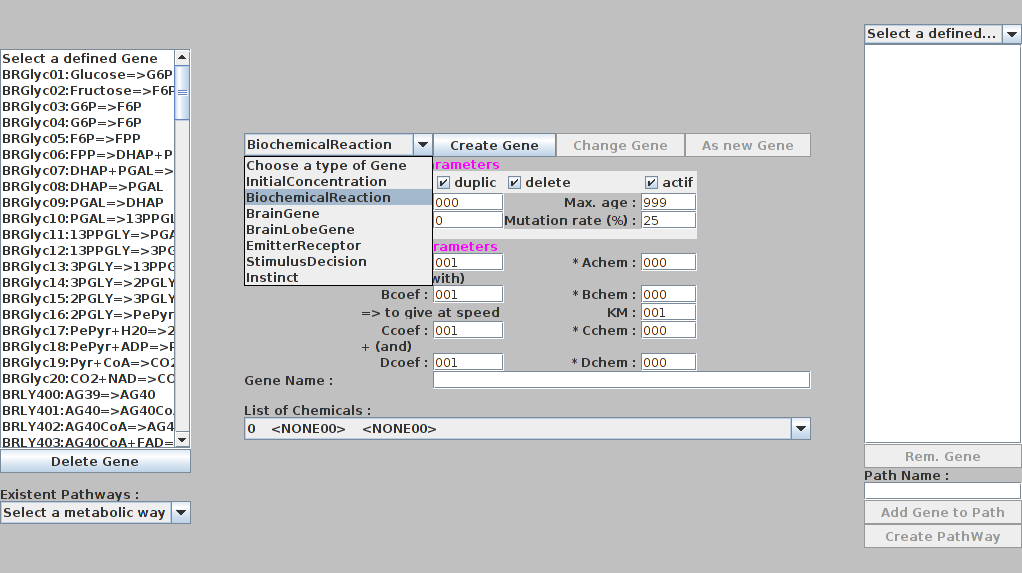
\includegraphics[height=6.5cm,width=11.6cm]{img/persoGeneCreatorGUI.png} \hfill\null
	% \vfill
\end{frame}

\subsubsection{\sectionPartIIcDE}
\begin{frame}
	\frametitle{\moreInFrameTitle \sectionPartIIcDE}
	\begin{center}
	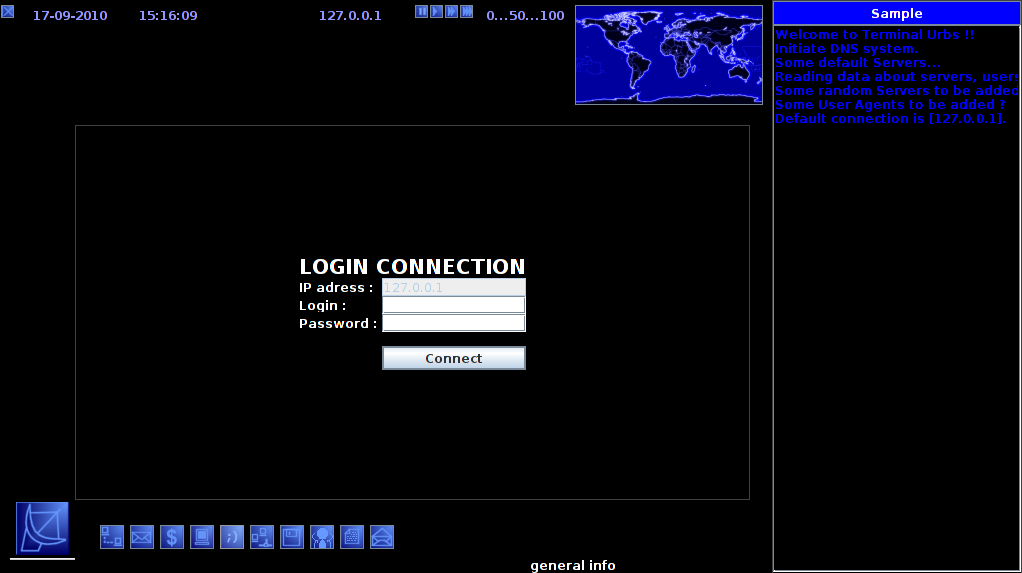
\includegraphics[height=6.5cm,width=11.6cm]{img/persoUplinkTerminalUrbs.png} 
	\end{center}
	% \vfill
	% \null\hfill 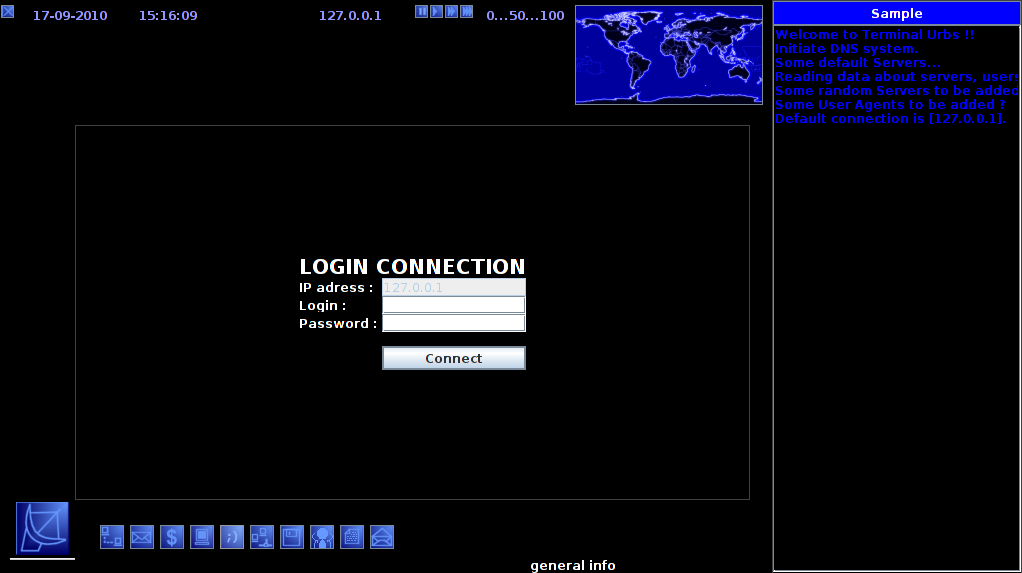
\includegraphics[height=6.5cm,width=11.6cm]{img/persoUplinkTerminalUrbs.png} \hfill\null
	% \vfill
\end{frame}

\subsubsection{\sectionPartIIcTR}
\begin{frame}
	\frametitle{\moreInFrameTitle \sectionPartIIcTR}
	\begin{center}
	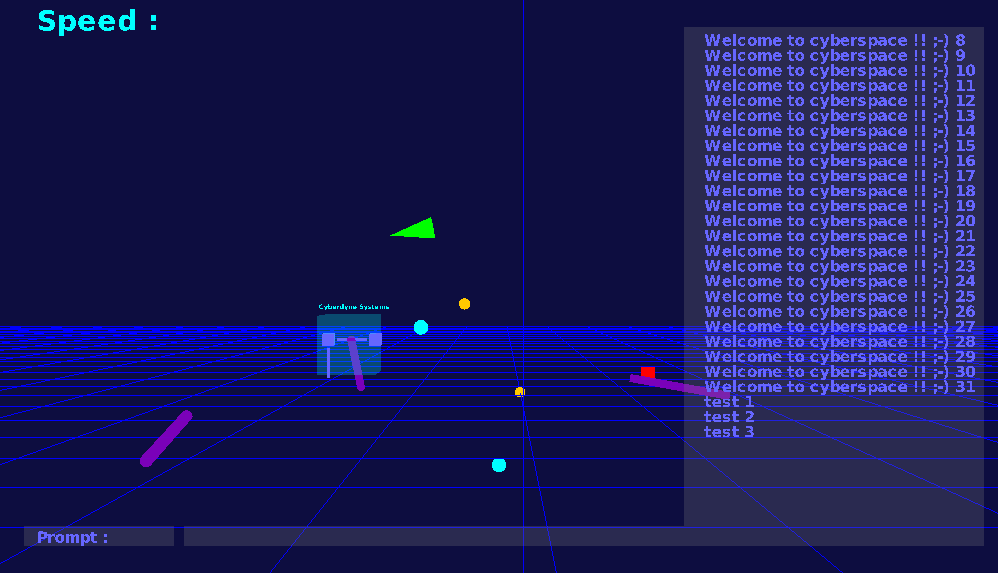
\includegraphics[height=6.5cm,width=11.6cm]{img/persoCyberSpaceInterweb.png} 
	\end{center}
	% \vfill
	% \null\hfill 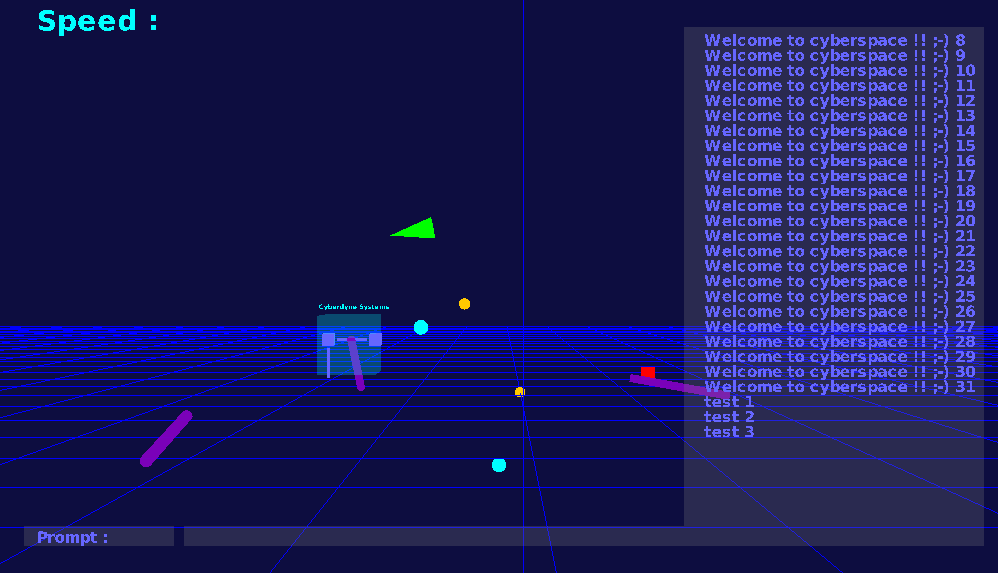
\includegraphics[height=6.5cm,width=11.6cm]{img/persoCyberSpaceInterweb.png} \hfill\null
	% \vfill
\end{frame}

%***************************************
%******     I Th{\'e}matique  	*******
%***************************************

\section{\sectionPartI}
\begin{frame}
	\frametitle{\moreInFrameTitle \sectionPartI}
	\tableofcontents[sections=2,subsectionstyle=shaded/shaded/shaded]
\end{frame} 

\subsection{\sectionPartIa}
\begin{frame}
	\frametitle{\moreInFrameTitle \sectionPartIa }
	\tableofcontents[sections=2,subsectionstyle=show/shaded/hide]
\end{frame} 

\subsubsection{\sectionPartIaUN}
\begin{frame}
	\frametitle{\moreInFrameTitle \sectionPartIaUN (1)}
	\begin{itemize}
		\item \underline{Conception} : {\'e}tablir un \textbf{cahier des charges} : 
			\begin{itemize}
				\item Rassembler les id{\'e}es, concepts...
				\item Organiser et planifier un ou plusieurs projets. 
				\item \texttt{Papier, crayons} ou {\'e}quivalents. 
			\end{itemize}
		\item \textbf{Diagrammes UML} (\emph{Unified Modeling Language}) : 
			\begin{itemize}
				\item Un dessin vaut parfois mieux qu'un long discours, avec (ou sans) explication(s). 
				\item Tableau(x) r{\'e}capitulatif(s) d'exemples de donn{\'e}es ou de nomenclature. 
				\item Diff{\'e}rents aspects d'un m{\^e}me probl{\`e}me et de sa r{\'e}solution. 
				\item \textbf{Classes, Cas d'utilisation, S{\'e}quence, Activit{\'e}s...}
			\end{itemize}
		\item \textbf{Design Patterns} : \emph{r{\'e}fl{\'e}chir {\`a} l'impl{\'e}mentation sans {\'e}crire une seule ligne de code !}
		\item \textbf{MVC} : \emph{Mod{\`e}le-Vue-Contr{\^o}lleur}, et \textbf{API} : \emph{Application Programming Interface} : r{\'e}flexion sur la s{\'e}paration des composants, ce qui interviendra lors du d{\'e}veloppement (modules, packages, GUI utilisateurS...). 
	\end{itemize}
\end{frame} 

\begin{frame}
	\frametitle{\moreInFrameTitle \sectionPartIaUN (2)}
	\textbf{\large{Les diagrammes UML}}
	\begin{columns}[c]
		\begin{column}[c]{5cm}
			\begin{alertblock}{Le diagramme de Classes}
			\end{alertblock}
			
			\begin{exampleblock}{Le diagramme de S{\'e}quences}
			\end{exampleblock}
		\end{column}
		\begin{column}[c]{5cm}
			\begin{exampleblock}{Le diagramme de Cas d'Utilisation}
			\end{exampleblock}
			
			\begin{alertblock}{Le diagramme d'{\'E}tat et / ou d'Activit{\'e}s}
			\end{alertblock}
		\end{column}
	\end{columns}
	Autres Diagrammes UML : {\'E}tat-Transition ; Composants ; Communication ; Structures composites...
\end{frame} 

\begin{frame}
	\frametitle{\moreInFrameTitle \sectionPartIaUN (4)}
	\textbf{Le diagramme de Classes}
	%% ici une image
	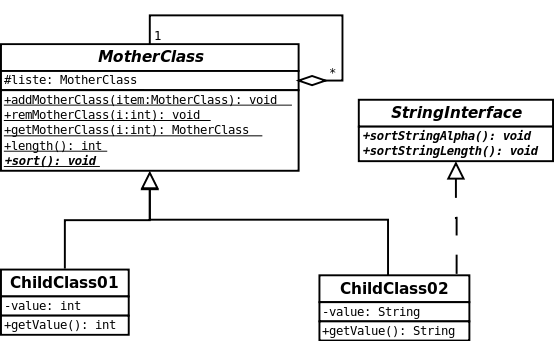
\includegraphics[height=6.5cm]{img/diagrammeClasses.png}	
\end{frame} 

\begin{frame}
	\frametitle{\moreInFrameTitle \sectionPartIaUN (5)}
	\textbf{Le diagramme de Cas d'Utilisation}
	%% ici une image
	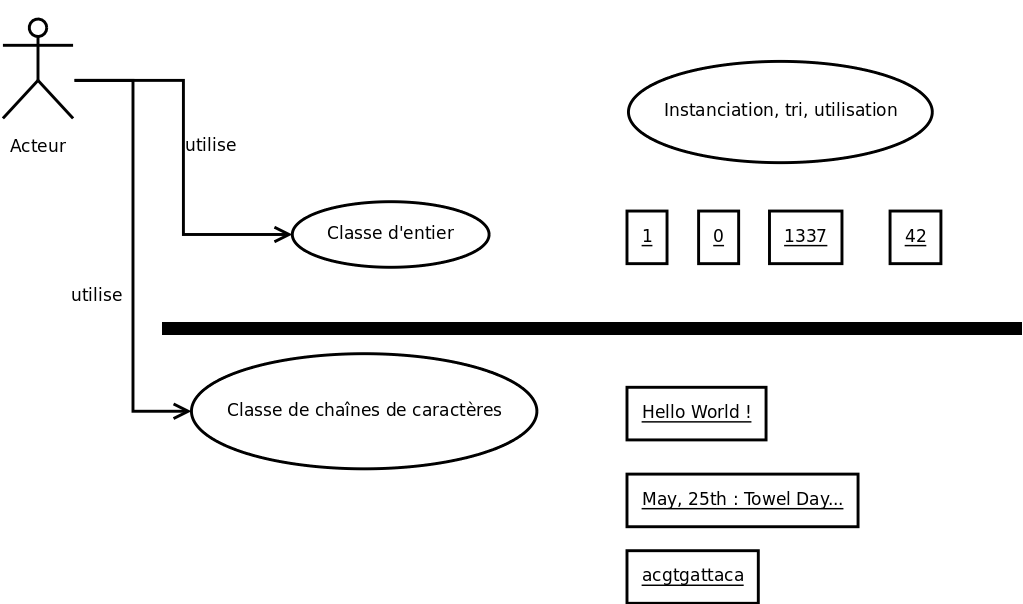
\includegraphics[height=6.5cm]{img/diagrammeCasUtilisation.png}
\end{frame} 

\begin{frame}
	\frametitle{\moreInFrameTitle \sectionPartIaUN (6)}
	\textbf{Le diagramme de S{\'e}quences}
	%% ici une image
	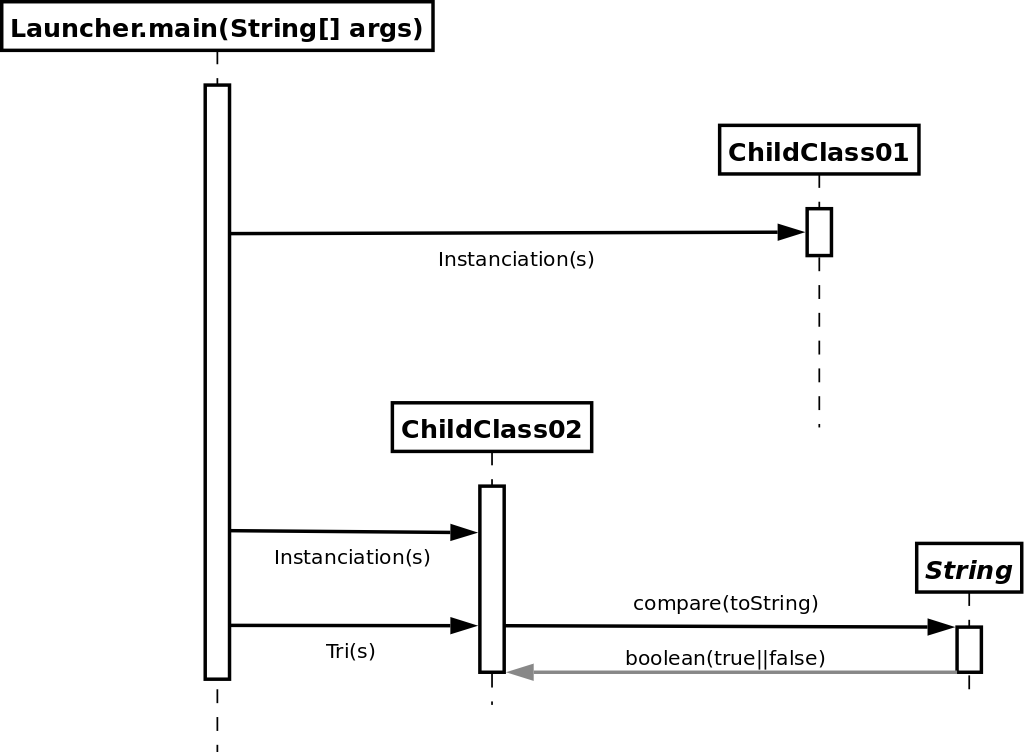
\includegraphics[height=6.5cm]{img/diagrammeSequence.png}
\end{frame} 

\begin{frame}
	\frametitle{\moreInFrameTitle \sectionPartIaUN (7)}
	\textbf{Le diagramme d'{\'E}tat et / ou d'Activit{\'e}s}
	%% ici une image
	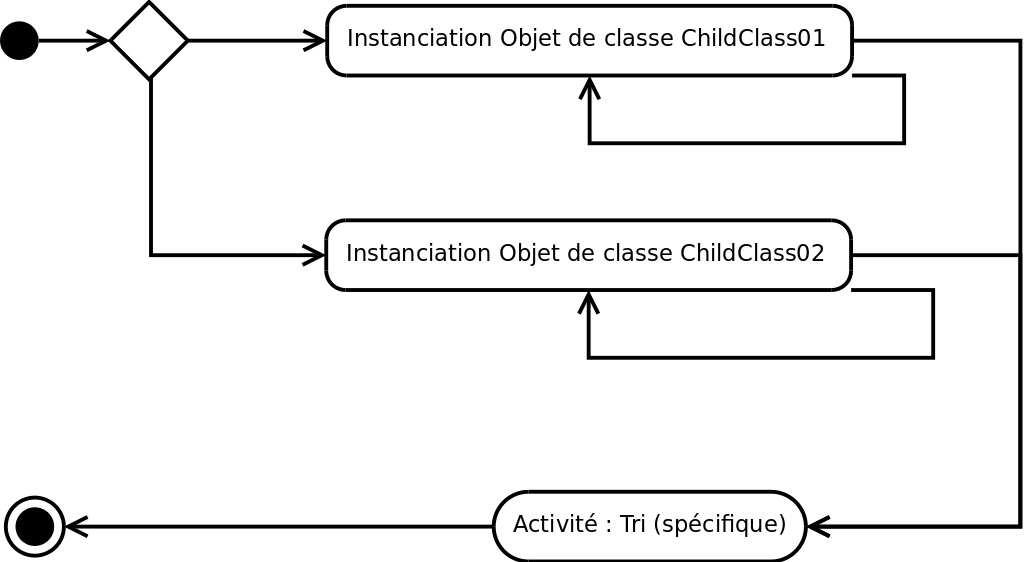
\includegraphics[height=6.0cm]{img/diagrammeEtatActivite.png}
\end{frame} 

\begin{frame}
	\frametitle{\moreInFrameTitle \sectionPartIaUN (8)}
	\textbf{\large{Les Design-Pattern's}}
	\begin{columns}[c]
		\begin{column}[c]{5cm}
			\begin{exampleblock}{Regroupements}
			\begin{itemize}
				\item Interfaces (cf. Structures)
				\item Responsabilit{\'e} (cf. Comportement)
				\item Construction (cf. Cr{\'e}ation)
				\item Op{\'e}rations
				\item Extensions
			\end{itemize}
			\end{exampleblock}
			\begin{alertblock}{Cr{\'e}ation}
			\begin{itemize}
				\item Abstractions et h{\'e}ritage
				\item Factorisation, 
				\item Builder,Prototype...
			\end{itemize}
			\end{alertblock}
		\end{column}
		\begin{column}[c]{5cm}
			\begin{alertblock}{Structure}
			\begin{itemize}
				\item Granularit{\'e} des classes et instances (Flyweight),
				\item Acc{\`e}s aux instances (Bridge, Fa\c{c}ade...),
				\item Adapter...
			\end{itemize}
			\end{alertblock}
			
			\begin{exampleblock}{Comportements}
			\begin{itemize}
				\item It{\'e}ration, 
				\item M{\'e}diation, 
				\item Cha{\^i}nes / Responsability...
			\end{itemize}
			\end{exampleblock}
		\end{column}
	\end{columns}
\end{frame} 

\subsubsection{\sectionPartIaDE}
\begin{frame}
	\frametitle{\moreInFrameTitle \sectionPartIaDE}
	\begin{enumerate}
		\item Documentation (besoins, cahier des charges, notes, diagrammes...). 
		\item Impl{\'e}mentation (documentation interne). 
		\item Tests (unitaires, {\'e}labor{\'e}s...). 
		\item Du \emph{Back Office} au \emph{Front Office} : rapports de bugs, re-impl{\'e}mentation, nouveaux besoins... 
		\item \emph{Industrialisation (utilisation courante, conditions logicielles et / ou mat{\'e}rielles...). }
		\item \emph{(Pr{\'e}-)Production et mise en service...}
	\end{enumerate}~\\
	Plus de d{\'e}tails dans le slide suivant et la partie suivante (\emph{\sectionPartId}). 
\end{frame} 

\subsubsection{\sectionPartIaTR}
\begin{frame}
	\frametitle{\moreInFrameTitle \sectionPartIaTR}
	\textbf{Partie finale} du cycle en V ou Y (retour vers une re-d{\'e}finition ou ajout de besoins, fonctionnalit{\'e}s... pour une correstion de bug ou une version suivante !). 
	
	\begin{columns}[c]
	\begin{column}[c]{6cm}
		\begin{beamerboxesrounded}	[lower=substructureTR, %
		 				 upper=block title TR,%
						 shadow=true]%
		       {Industrialisation}
		        \begin{itemize}
				\item Modifier l'impl{\'e}mentation pour une utilisation courante
				\item Enlever (ou rendre inaccessibles) les parties de tests. 
				\begin{itemize}
					\item les parties de tests, 
					\item le code source (propri{\'e}taire ; libre, ouvert...). 
				\end{itemize}
				\item Facile {\`a} (re-)installer (version via CVS / SVN -- \textbf{subversion}). 
			\end{itemize}
		 \end{beamerboxesrounded}
	\end{column}
	\begin{column}[c]{6cm}
		 \begin{beamerboxesrounded}	[lower=substructureDE, %
		 				 upper=block title DE,%
						 shadow=true]%
		       {(Pr{\'e}-)Production}
		        \begin{itemize}
				\item Tests en grandeur / taille r{\'e}elle. 
				\item Mise en fonctionnement courant (\emph{Front Office}). 
				\item Distribution aupr{\`e}s de l'utilisateur (installation). 
				\item Accessibilit{\'e} aupr{\`e}s de l'utilisateur (service web...). 
			\end{itemize}
		 \end{beamerboxesrounded}
		 
	\end{column}
	\end{columns}
\end{frame}

\subsection{\sectionPartId}
\begin{frame}
	\frametitle{\moreInFrameTitle \sectionPartId}
	\tableofcontents[sections=2,subsectionstyle=show/shaded/hide]
\end{frame} 

\subsubsection{\sectionPartIdUN}
\begin{frame}
	\frametitle{\moreInFrameTitle \sectionPartIdUN -- 1}
	\begin{itemize}
		\item \textbf{Environnements de D{\'e}veloppements Int{\'e}gr{\'e}s} : outils d'aides. 
		\begin{enumerate}
			\item Conception, d{\'e}veloppement. 
			\item Mod{\`e}les de classes et packages. 
			\item Reconnaissance de langage(s) et mise en valeurs de mots-cl{\'e}s. 
			\item Signaux d'avertissements, d'erreurs...
		\end{enumerate}
		\item Modules compl{\'e}mentaires (pour Eclipse : Subclipse, EPIC, C / C++, PyDev, XML...) et autres IDE (xCode, Visual Studio...). 
		\item Gestion du temps, projet(s), versions (SVN), Int{\'e}gration de m{\'e}thodes de gestion de projets.
	\end{itemize}
\end{frame}

\begin{frame}
	\frametitle{\moreInFrameTitle \sectionPartIdUN -- 2}
	\begin{itemize}		
		\item \textbf{"D{\'e}marche qualit{\'e}"}
		\begin{enumerate}
			\item {\'E}crire et d{\'e}crire ce que l'on fait et r{\'e}alise. 
			\item Validation progressive (points de blocage, points r{\'e}alis{\'e}s, erreurs connues...). 
			\item Des normes ISO existent (9000-9100 pour la d{\'e}marche qualit{\'e}, 9100-9999 pour les langages, 27000 pour la s{\'e}curit{\'e} des informations...). 
		\end{enumerate}
		\item Beaucoup de documentation supl{\'e}mentaire mais ajoute la v{\'e}rification. 
		\item \emph{Outil facultatif / optionnel. }
	\end{itemize}
\end{frame} 

\subsubsection{\sectionPartIdDE}
\begin{frame}
	\frametitle{\moreInFrameTitle \sectionPartIdDE  -- 1}
	\begin{columns}[c]
	\begin{column}[c]{6cm}
		 \begin{beamerboxesrounded}	[lower=substructureDE, %
		 				 upper=block title DE,%
						 shadow=true]%
		       {Quelques indications...}
			\begin{itemize}
				\item eXtreme Programming : 
				\begin{itemize}
					\item It{\'e}rations, 
					\item alternance documentation et impl{\'e}mentation. 
				\end{itemize}
				\item M{\'e}thode Scrum. 
				\begin{itemize}
					\item Cycle de d{\'e}veloppement (sur une semaine / un mois). 
					\item Travail en {\'e}quipe (r{\'e}partition dans le temps et entre membres). . 
				\end{itemize}
				\item M{\'e}thodes "agiles" (adaptation). 
				\item \textbf{Versions successives. }
			\end{itemize}
		\end{beamerboxesrounded}
	\end{column}
	\begin{column}[c]{6cm}
		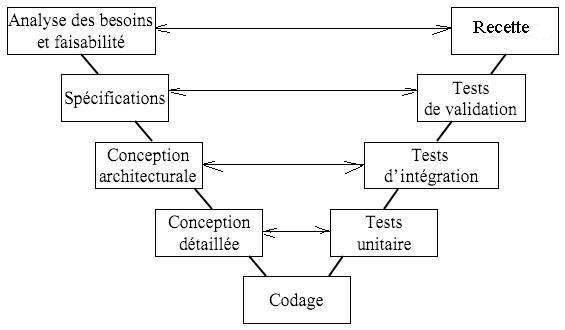
\includegraphics[width=6cm]{img/Cycle_de_developpement_en_v.png}~\\
		\begin{center} \emph{Le cycle en V, un classique...} \end{center}
	\end{column}
	\end{columns}~\\
	Voir notamment \emph{http://fr.wikipedia.org/wiki/Scrum\_(methode)} ainsi que les articles ET r{\'e}f{\'e}rences li{\'e}s. 
\end{frame}

\begin{frame}
	\frametitle{\moreInFrameTitle \sectionPartIdDE -- 2}
		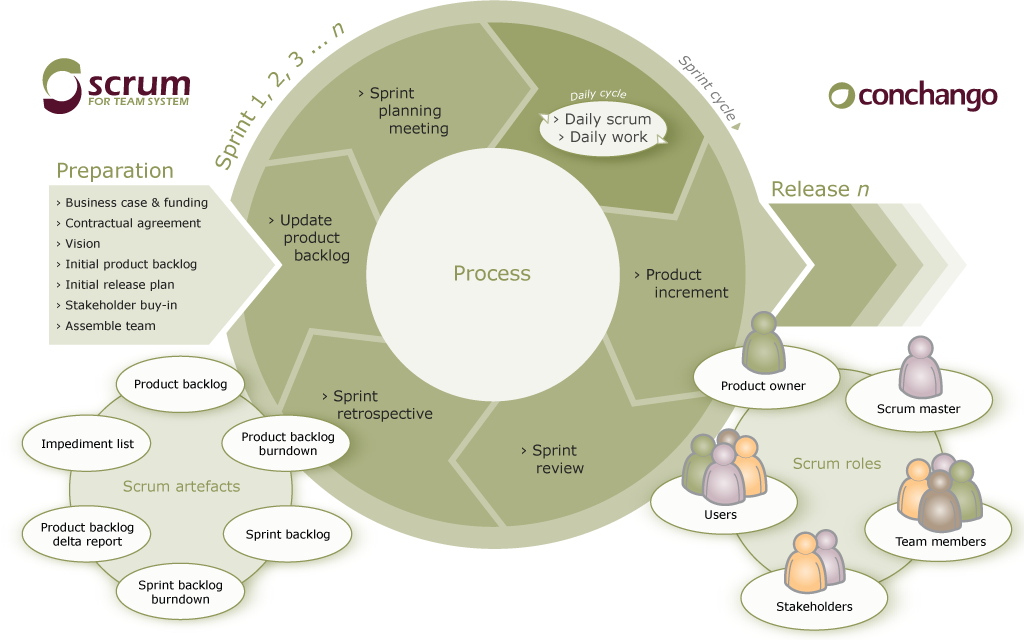
\includegraphics[width=10cm]{img/Scrum-Overview-Diagram.png}~\\
		\begin{center} \emph{Le d{\'e}roulement de SCRUM : {\'e}tapes du cycle. } \end{center}
\end{frame}

\subsubsection{\sectionPartIdTR}
\begin{frame}
	\frametitle{\moreInFrameTitle \sectionPartIdTR}
	\begin{columns}[T]
	\begin{column}[T]{7cm}
		\begin{footnotesize} \textbf{Pour quoi se compliquer la vie ?} \end{footnotesize}
		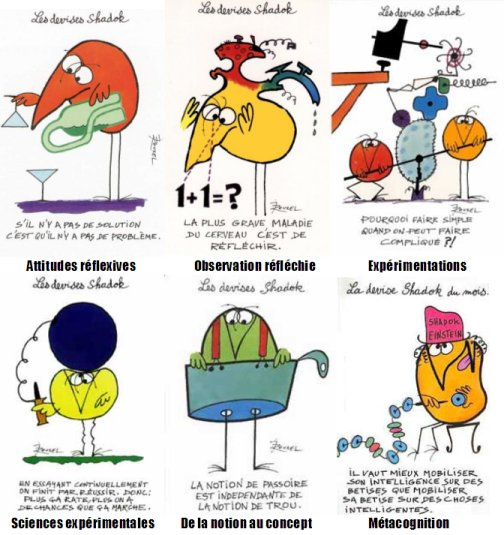
\includegraphics[width=7cm]{img/shadoks_devises.png}~\\
		% \begin{center} \emph{Le cycle en V, un classique...} \end{center}
	\end{column}
	\begin{column}[T]{5.5cm}
		\begin{itemize}
			\item Faisabilit{\'e} / Prototype : preuve de concept (en d{\'e}but de projet). 
			\item Industrialiser : faire fonctionner couramment. 
			\item Pouvoir faire {\'e}voluer le projet sans tout refaire. 
			\item L'effet (besoin) n'est pas ind{\'e}pendant de la faisabilit{\'e} de la cause (r{\'e}ponse). 
			\item \textbf{Projets mal con\c{c}us donc non maintenables, jet{\'e}s...}
			\item \emph{{\'E}viter le coin de table (projet et douleur). }
		\end{itemize}
	\end{column}
	\end{columns}~\\
\end{frame} 

\subsection{\sectionPartIb}
\begin{frame}
	\frametitle{\moreInFrameTitle \sectionPartIb}
	\tableofcontents[sections=2,subsectionstyle=show/shaded/hide]
\end{frame} 

\subsubsection{\sectionPartIbUN}
\begin{frame}
	\frametitle{\moreInFrameTitle \sectionPartIbUN}
	\begin{columns}[t]
	\begin{column}[c]{6cm}
		\begin{beamerboxesrounded}	[lower=substructureUN, %
		 				 upper=block title UN,%
						 shadow=true]%
		       {Formats de fichiers !!}
		        \begin{enumerate}
				\item Fichiers "plats" : texte brut ; tabulaire, structuration sp{\'e}cifique, scripts...
					\begin{itemize} \item FASTA, EMBL, GenBank... \end{itemize}
				\item Fichiers XML : semi-structuration, d{\'e}finition (DTD, XSD). 
					\begin{itemize} \item UniprotKB... \end{itemize}
				\item Fichiers binaires (issus de compilation, instances s{\'e}rialis{\'e}es...). 
				\item R{\'e}pertoires, liens symboliques (via le syst{\`e}me d'exploitation)...
				\item Bases De Donn{\'e}es (selon SGBD). 
			\end{enumerate}
		 \end{beamerboxesrounded}
	\end{column}
	\begin{column}[c]{6cm}
		 \begin{beamerboxesrounded}	[lower=substructureTR, %
		 				 upper=block title TR,%
						 shadow=true]%
		       {Extraction de donn{\'e}es, conversions...}
		        \begin{itemize}
				\item \emph{Parsers} pr{\'e}-existants (BioPerl, BioPython...)
				\item Moteurs d'extractions g{\'e}n{\'e}riques (pour le XML si d{\'e}finition, XPath). 
				\item SGBD : MySQL, Postgre, Oracle $\rightarrow$ particularismes. 
				\item Construire son propre syst{\`e}me d'extraction de donn{\'e}es (autant voire plus de temps {\`a} utiliser). 
			\end{itemize}
		 \end{beamerboxesrounded}
	\end{column}
	\end{columns}
\end{frame} 

\subsubsection{\sectionPartIbDE}
\begin{frame}
	\frametitle{\moreInFrameTitle \sectionPartIbDE}
	\begin{itemize}		 
		\item \textbf{Int{\'e}r{\^e}t : } structurer et trouver facilement une donn{\'e}e selon certains crit{\`e}res, autrement que par un \emph{find} ou un \emph{grep} ou tout autre {\'e}quivalent...~\\
		\item \textbf{Optimisation} du stockage de donn{\'e}es en volum{\'e}trie et en liens (XML tr{\`e}s verbeux et redondant, fichiers plats faiblement reli{\'e}s entre eux...), mais peut {\^e}tre moins efficace (rare). 
		\item Couplage {\`a} une ou plusieurs interfaces utilisateurs / programmes via des connecteurs sp{\'e}cifiques (PHP, Python, Perl, Java...). 
		\item \textbf{Entit{\'e}s-Relations} et SQL : int{\'e}r{\^e}t et utilit{\'e} de UML. 
		\begin{itemize}
			\item Bien d{\'e}finir les entit{\'e}s et leurs liens. 
			\item {\'E}viter les confusions {\`a} venir sur l'utilisation de(s) la base(s) de donn{\'e}es (sch{\'e}ma, table, colonne). 
		\end{itemize}
	\end{itemize}
\end{frame} 

\subsubsection{\sectionPartIbTR}
\begin{frame}
	\frametitle{\moreInFrameTitle \sectionPartIbTR}
	\begin{itemize}	
		\item \underline{Choix d'impl{\'e}mentation : } quantit{\'e} de donn{\'e}es, r{\'e}partition, utilisation, codage, rapidit{\'e}, enregistrement, m{\'e}moire...
		\item \textbf{Berkeley} : couples (clef;valeur) et structures similaires. 
		\item \textbf{\underline{SGBDR}} : le plus classique (SQL). 
		\item \textbf{SGBDO} : du Relationnel {\`a} l'Objet : lourd et peu utilis{\'e} (s{\'e}rialization d'instances d'objets). 
		\item \textbf{ORM} -- \underline{Object-Relationnal-Mapping} : relier une Programmation Objet et un SGBDR sans {\'e}crire du SQL !!
	\end{itemize}
\end{frame} 


\subsection{\sectionPartIc}
\begin{frame}
	\frametitle{\moreInFrameTitle \sectionPartIc}
	\tableofcontents[sections=2,subsectionstyle=show/shaded/hide]
\end{frame} 

\subsubsection{\sectionPartIcUN}
\begin{frame}
	\frametitle{\moreInFrameTitle \sectionPartIcUN}
	\begin{itemize}	
		\item \textbf{Int{\'e}r{\^e}t : } Cha{\^i}nes de traitement ETL (Extraction, Traitement, Chargement)
		\item \textbf{Langages : } Perl, Python, Shell et d{\'e}riv{\'e}s (bash, ksh...). 
		\item L'objectif est ici la rapidit{\'e} de traitement dans la conversion des donn{\'e}es, la Programmation Orient{\'e}e Objet est \emph{facultative} dans ce cas. 
		\item Aide d'outils adapt{\'e}s : \emph{ImageMagick} pour les images, \emph{gs} pour les PDF, \emph{libxml}...). 
		\item Utilisation de l'ordinateur comme d'un automate avec une grosse m{\'e}moire ({\'e}v{\`e}nements, base de donn{\'e}es...). 
	\end{itemize}
\end{frame} 

\subsubsection{\sectionPartIcDE}
\begin{frame}
	\frametitle{\moreInFrameTitle \sectionPartIcDE}
	\begin{itemize}	
		\item \textbf{Int{\'e}r{\^e}t : } Repr{\'e}sentation des donn{\'e}es et leur manipulation. 
		\item \textbf{Langages : } Java, C++, PHP5...
		\item Indispensable pour bien conceptualiser !!
		\item Code compr{\'e}hensible humainement, maintenable, factorisable... 
		\item Structures communes (h{\'e}ritage, interfaces, Design-Patterns). 
		\item \textbf{Repr{\'e}sentation, Classification, Manipulation !!}
		\item Comme pour repr{\'e}sentation ER : \emph{si on ne comprend pas bien, ne pas faire...}
	\end{itemize}
\end{frame} 

\subsubsection{\sectionPartIcTR}
\begin{frame}
	\frametitle{\moreInFrameTitle \sectionPartIcTR}
	\begin{enumerate}
		\item \emph{Trigger} de Bases De Donn{\'e}es
		\begin{itemize}	
			\item \textbf{Int{\'e}r{\^e}t : } fonctions construites en BDD pour la manipulation des donn{\'e}es. 
			\item \textbf{Langages : } SQL, C...
		\end{itemize}
		\item XSLT
		\begin{itemize}	
			\item \textbf{Int{\'e}r{\^e}t : } Manipulation directe des donn{\'e}es dans leur(s) format(s). 
			\item \textbf{Langages : } XML. 
		\end{itemize}
		\item Documentation : Wiki, \LaTeX, Code Source...
		\begin{itemize}	
			\item \textbf{Int{\'e}r{\^e}ts : } relecture du code, reprise du projet, maintenabilit{\'e} du projet et du code source...
			\item \textbf{Langages : } \TeX / \LaTeX, RST, JavaDoc et assimil{\'e}s, .... 
			\item \textsc{\textbf{Indispensable !!}}
		\end{itemize}
	\end{enumerate}
\end{frame} 


%***************************************
%******     III <<Pack Bonus>>   *******
%***************************************
\section{\sectionPartIII}
\begin{frame}
	\frametitle{\moreInFrameTitle \sectionPartIII}
	\tableofcontents[sections=3,subsectionstyle=shaded/shaded/shaded]
\end{frame} 

\subsection{\sectionPartIIIa}
\begin{frame}
	\frametitle{\moreInFrameTitle \sectionPartIIIa}
	\tableofcontents[sections=3,subsectionstyle=show/shaded/hide]
\end{frame} 

\subsubsection{\sectionPartIIIaUN}
\begin{frame}
	\frametitle{\moreInFrameTitle \sectionPartIIIaUN}
	\begin{itemize}
		\item Librairie R{\'e}elles ET Logicielles \emph{explorer / tester}.  
		\item \emph{En BioInfo} BioPerl, BioPython, BioJava, BioC++...
		\item {\footnotesize \emph{http://www.dmoz.org/Science/Biology/Bioinformatics/Software/} }
		\item Encyclop{\'e}dies : p{\'e}rim{\'e}es d{\`e}s la publication : \underline{\emph{approfondir}}. 
	\end{itemize}~\\
	\begin{center}
	
\includegraphics[width=3cm]{img/logo_wikipedia.png}~\\ 
	\emph{Un point de d{\'e}part, \underline{ne pas s'en contenter},~\\ y participer {\'e}ventuellement. }
	\end{center}
\end{frame} 

\subsubsection{\sectionPartIIIaDE}
\begin{frame}
	\frametitle{\moreInFrameTitle \sectionPartIIIaDE}
	\begin{center}
	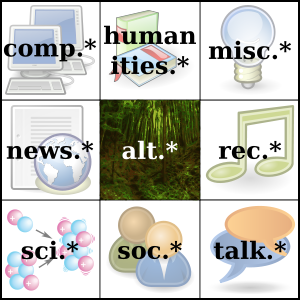
\includegraphics[width=3cm]{img/usenet-hierarchie.png}~\\ 
	\emph{UseNet et NewsGroups : posez des questions, r{\'e}pondez-y aussi !! }
	\end{center}
	\textbf{La liste bioinfo : \emph{http://listes.sfbi.fr/wws/info/bioinfo} }~\\
	Groupes UseNet et Google Groups (Listes Python et Perl). ~\\
	\begin{itemize}
		\item \emph{http://www.usenet-fr.net/} : \texttt{fr.usenet.usages}, \texttt{fr.sci.biologie}...
		\item \texttt{sci.bio.technology}, \texttt{bionet.celegans}, \texttt{alt.bio.ethics}, \texttt{alt.bio.hackers}...
		\item \emph{http://news.lacave.net/servers/reader/list}
	\end{itemize}
\end{frame} 

\subsubsection{\sectionPartIIIaTR}
\begin{frame}
	\frametitle{\moreInFrameTitle \sectionPartIIIaTR}
	\begin{itemize}
		\item<1-> Faire l'effort de s'informer, m{\^e}me de fa\c{c}on passive (e-mail, newsgroup, RSS, journaux...) : cas pr{\'e}c{\'e}dents. 
		\item<2-> M{\'e}thodologie active (exemples) : 
		\begin{itemize}
			\item maintenir une bibliographie, si possible {\`a} jour, {\'e}tendue (sources primaires et secondaires). 
			\item tenir un journal ou un blog (\emph{DLFP}, \emph{http://duvernoisevelyne.blog.rhonealpesjob.com/}, \emph{http://www.biologeek.com/})...
		\end{itemize}
		\item<3-> Vitae $ \neq $ Mortae : maintenir son Curriculum {\`a} jour. 
		\item<3-> Informer (journal, blog : acc{\`e}s public ou restreint). 
	\end{itemize}
\end{frame}

\subsection{\sectionPartIIIb}
\begin{frame}
	\frametitle{\moreInFrameTitle \sectionPartIIIb}
	\tableofcontents[sections=3,subsectionstyle=show/shaded/hide]
\end{frame} 

\subsubsection{\sectionPartIIIbUN}
\begin{frame}
	\frametitle{\moreInFrameTitle \sectionPartIIIbUN}
	\begin{columns}[c]
	\begin{column}[c]{7cm}
		 \begin{beamerboxesrounded}	[lower=substructureUN, %
		 				 upper=block title UN,%
						 shadow=true]%
		       {\sectionPartIIIbUN}
			\begin{itemize}
				\item Dipl{\^o}me : reconnaissance ultime ?
				\begin{itemize}
					\item Pas forc{\'e}ment demand{\'e} dans le priv{\'e} (exp{\'e}rience ET p{\'e}riode d'essai). 
					\item Un projet de trois ans vaut bien un doctorat, un dipl{\^o}me d'ing{\'e}nieur, une comp{\'e}tence acquise...
				\end{itemize}
				\item Apprentissage permanent (curiosit{\'e}, formations diplomantes ou non...). 
				\item \emph{L'attitude n'est pas un substitut {\`a} la comp{\'e}tence. }
			\end{itemize}
		\end{beamerboxesrounded}
	\end{column}
	\begin{column}[c]{4cm}
		
\includegraphics[width=4cm]{img/yodaInCloneWars.png}~\\
	\end{column}
	\end{columns}
\end{frame} 

\subsubsection{\sectionPartIIIbDE}
\begin{frame}
	\frametitle{\moreInFrameTitle \sectionPartIIIbDE}
	\begin{columns}[c]
	\begin{column}[c]{5cm}
		
\includegraphics[width=4cm]{img/nocomicsans.png}~\\
		{\footnotesize \emph{Respect des normes et standards. } }~\\
	\end{column}
	\begin{column}[c]{7cm}
		 \begin{beamerboxesrounded}	[lower=substructureDE, %
		 				 upper=block title DE,%
						 shadow=true]%
		       {\sectionPartIIIbDE}
			\begin{itemize}
				\item<2-> \textbf<2-3>{HackerSpaces. }
				\begin{itemize}
					\item Lieux de partages (information, {\'e}lectronique...). 
					\item Do It Yourself (prototypage, manuels...). 
					\item DIY Bio (essor actuel : mat{\'e}riel, {\'e}thique...). 
					\item \textbf{/tmp/lab} \emph{http://www.tmplab.org/}
				\end{itemize}
				\item<3-> Projets et initiatives personnels. 
				\item<4-> Logiciels Libres // Open Source. 
				\item<4-> "Biologie Libre // Open Source". 
			\end{itemize}
		\end{beamerboxesrounded}
	\end{column}
	\end{columns}
\end{frame} 

\subsubsection{\sectionPartIIIbTR}
\begin{frame}
	\frametitle{\moreInFrameTitle \sectionPartIIIbTR}
	\begin{columns}[c]
	\begin{column}[c]{7cm}
		 \begin{beamerboxesrounded}	[lower=substructureTR, %
		 				 upper=block title TR,%
						 shadow=true]%
		       {\sectionPartIIIbTR}
			\begin{itemize}
				\item<1-> <<Homologies>> entre les deux (syst{\`e}mes complexes, fonctionnement...). 
				\item<2-> Comp{\'e}tences d'analyse, de conception. 
				\item<2-> Aspects scientifiques $ >> $ purement informatique... 
				\item<3-> Construction mutuelle (limitations techniques et usages). 
				\item<4-> (\emph{Steve Jobs}) : s'il d{\'e}marrait Apple maintenant ce serait dans les biotech's... 
			\end{itemize}
		\end{beamerboxesrounded}
	\end{column}
	\begin{column}[c]{4cm}
		
\includegraphics[width=4cm]{img/bioinformatique.png}~\\
	\end{column}
	\end{columns}
\end{frame} 

\subsection{\sectionPartIIIc}
\begin{frame}
	\frametitle{\moreInFrameTitle \sectionPartIIIc}
	\tableofcontents[sections=3,subsectionstyle=show/shaded/hide]
\end{frame} 

\subsubsection{\sectionPartIIIcUN}
\begin{frame}
	\frametitle{\moreInFrameTitle \sectionPartIIIcUN}
	\begin{columns}[c]
	\begin{column}[c]{7cm}
		\begin{beamerboxesrounded}	[lower=substructureUN, %
		 				 upper=block title UN,%
						 shadow=true]%
			{\sectionPartIIIcUN}
			\begin{itemize}
				\item Universit{\'e} et recherche fran\c{c}aise, financements (voir : Angleterre, Allemagne). 
				\item Liens public-priv{\'e} (ad{\'e}quation des formations et des comp{\'e}tences). 
				\begin{itemize}
					\item Construction mutuelle (limitations techniques et usages). 
					\item Soutiens mutuels (formations, ressources). 
				\end{itemize}
				\item Apprentissage personnel (autodidactes) et "privatisation de l'enseignement". 
			\end{itemize}
		\end{beamerboxesrounded}
	\end{column}
	\begin{column}[c]{4cm}
		
\includegraphics[width=4cm]{img/omnesDOCETubique.png}~\\
		\emph{Omnes Docet Ubique}~\\ \footnotesize{ \texttt{Enseigner {\`a} Tous et en Tous Lieux} ~\\ (Abb{\'e} Gr{\'e}goire 1794) }
	\end{column}
	\end{columns}
\end{frame} 

\subsubsection{\sectionPartIIIcDE}
\begin{frame}
	\frametitle{\moreInFrameTitle \sectionPartIIIcDE}
	\begin{itemize}
		\item<1-> \textbf<1-1>{Besoin pr{\'e}cis / ponctuels de recherche. }
		\begin{itemize}
			\item Faisabilit{\'e}, preuve de concept. 
			\item Marge de proposition / recherche fondamentale. 
		\end{itemize}
		\item<2-> \textbf<2-2>{Besoins {\`a} plus long terme. }
		\begin{itemize}
			\item Propositions industriel $ \Leftrightarrow $ (chercheur || {\'e}quipe). 
			\item Gestion en projets. 
			\item Financement direct. 
		\end{itemize}
		\item<3-> \textbf<3-3>{Formation} dans les entreprises. 
		\item<3-> Formation dans les centre de recherches. 
	\end{itemize}
\end{frame} 

\subsubsection{\sectionPartIIIcTR}
\begin{frame}
	\frametitle{\moreInFrameTitle \sectionPartIIIcTR}
	\begin{itemize}
		\item \textbf{En guise de conclusion...}
		\item ETL + Bases De Donn{\'e}es : toujours utile (quelque soit le domaine) : conception et d{\'e}veloppement permanent utile (base existante ou \emph{de novo)}. 
		\item Choix d'impl{\'e}mentation, changements...
		\item \emph{Le pr{\'e}sent n'est pas certain, l'avenir l'est moins} : initiative de groupe ou personnelle (profiter des deux). 
		\item Profitez de vos connaissances et de l'information dont vous disposez ! Mais ne vous limitez pas {\`a} cela...
	\end{itemize}
\end{frame} 


\section{\sectionPartIV}
\begin{frame}
	\frametitle{\moreInFrameTitle \sectionPartIV}
	{\centering \textbf{Questions} ?? }
\end{frame} 

\subsection{\sectionPartIVa}
\begin{frame}
	\frametitle{\moreInFrameTitle \sectionPartIVa}
	\begin{footnotesize}
	\begin{columns}[T]
	\begin{column}[T]{5cm}
		
\includegraphics[height=3cm]{img/tux.png}~\\~\\
		
\includegraphics[height=4cm]{img/Nuvola_apps_emacs.png}~\\~\\
	\end{column}
	\begin{column}[T]{7cm}
		\begin{beamerboxesrounded}	[lower=substructureDE, %
		 				 upper=block title DE,%
						 shadow=true]%
		       {\sectionPartIVa}
			\begin{itemize}
				\item Libre / Open Source : 4 libert{\'e}s fondamentales. 
				\begin{enumerate}
					\item La libert{\'e} d'utilisation, pour tous les usages [limitations {\'e}thiques]. 
					\item La libert{\'e} d'{\'e}tudier, pour adapter {\`a} ses besoins. 
					\item La libert{\'e} de redistribuer des copies (ou assimil{\'e} : cultures, lign{\'e}es). 
					\item La libert{\'e} d'am{\'e}liorer et de publier ces am{\'e}liorations pour la communaut{\'e}. 
				\end{enumerate}
				\item Licences libres (GPL, Creative Commons...), des droits de r{\'e}utilisation et re-publication. 
				\item Open Source : libert{\'e} de moyens (le logiciel est un outil). 
				\item \textbf{Int{\'e}r{\^e}t : } cadre formel (et non plus informel) de modificationS au sein de la communaut{\'e}. 
			\end{itemize}
		\end{beamerboxesrounded}
	\end{column}
	\end{columns}
	\end{footnotesize}
\end{frame}

\subsection{\sectionPartIVb}
\begin{frame}
	\frametitle{\moreInFrameTitle \sectionPartIVb}
	\begin{beamerboxesrounded}	[lower=substructureTR, %
					 upper=block title TR,%
					 shadow=true]%
	       {\sectionPartIVb}
		\begin{itemize}
			\item Commandes et outils classiques : \emph{ed / sed ; grep ; find ; ...} (se faire un memento -- aide-m{\'e}moire). 
			\item {\'E}diteurs de textes : vi ; emacs ; nano / pico / jedit ; geany ; Notepad++ ; ...
			\item {\'E}mulateurs : Wine ; qemu ; Virtual Box ; ...
			\item Outils en ligne de commande : mc (Midnight Commander) ; mutt ; screen / byobu ; ...
			\item IDE / Environnements de d{\'e}veloppement : Eclipse (et ses nombreux plug-ins / modules) ; {\'e}diteur de texte favori ++ compilateur(s) ; ...
			\item Outils de version : diff, patch, CVS, SVN (\textsc{subversion})...
			\item Traitement d'images, construction de diagrammes : \emph{ImageMagick}, GIMP, Dia, ArgoUML, Umbrello...
		\end{itemize}
	\end{beamerboxesrounded}
\end{frame}

\subsection{\sectionPartIVc}
\begin{frame}
	\frametitle{\moreInFrameTitle \sectionPartIVc}
	\begin{beamerboxesrounded}	[lower=substructureDE, %
					 upper=block title DE,%
					 shadow=true]%
	       {\sectionPartIVc}
		\begin{itemize}
			\item<1-> \textbf<1-1>{Contrats Public} : Vacataires (recrutement direct, temporaire) et permanent (fonctionnaire). 
			\item<1-> \textbf<1-1>{Contrats Priv{\'e}} : CDD / Int{\'e}rim (court, primes, conditions), CDI (p{\'e}riode d'essai). 
			\item<1-> \textbf<1-1>{Militaire} : contrats de 3 {\`a} 5 ans, conditions particuli{\`e}res. 
			\item<2-> \textbf<2-2>{Recherche d'emploi} : NO Bisounours !
			\item<2-> \textbf<2-2>{APEC}, P{\^o}le-Emploi (ex-ANPE) : d{\'e}p{\^o}t de CV gratuit / recherche de CV gratuite : cons{\'e}quences (budget, recrutement...). 
			\item<2-> \textbf<2-2>{Monster} : d{\'e}p{\^o}t de CV gratuit / recherche de CV {\`a} tarifs variables : diff{\'e}rents types de recrutement. 
			\item <2-> \textbf<2-2>{Candidature} spontan{\'e}e : faible taux de r{\'e}ponse, il faut correspondre aux attentes en cours (cf. listes sp{\'e}cialis{\'e}es). 
		\end{itemize}
	\end{beamerboxesrounded}
\end{frame}

\subsection{\sectionPartIVd}
\begin{frame}
	\frametitle{\moreInFrameTitle \sectionPartIVd}
	\begin{beamerboxesrounded}	[lower=substructureTR, %
					 upper=block title TR,%
					 shadow=true]%
	       {\sectionPartIVd}
		\begin{itemize}
			\item \textbf{Entretiens : } naturel mais neutre, pas oblig{\'e} de r{\'e}pondre {\`a} toutes les questions, faire le tri et s'entra{\^i}ner. 
			\item \textbf{Au boulot : } bien faire et efficace, prendre des pauses (mentales, physiques...), pr{\'e}parer au stress si besoin. 
			\item \underline{Savoir dire "NON"} : mettre des limites, conna{\^i}tres les siennes, r{\'e}partir vie pro. / vie priv{\'e}e...
			\item \emph{Mettre de l'argent de c{\^o}t{\'e}}, m{\^e}me un minimum : toujours utile, pr{\'e}parer l'avenir, logement, changer de boulot...
		\end{itemize}
	\end{beamerboxesrounded}
\end{frame}

\subsection{\sectionPartIVe}
\begin{frame}
	\frametitle{\moreInFrameTitle \sectionPartIVe}
	{\centering \textbf{Questions} ?? }
\end{frame} 



\end{document}
